\documentclass[10pt,twocolumn,letterpaper]{article}

\usepackage{cvpr}
\usepackage{times}
\usepackage{epsfig}
\usepackage{graphicx}
\usepackage{amsmath}
\usepackage{amssymb}

% Include other packages here, before hyperref.

% If you comment hyperref and then uncomment it, you should delete
% egpaper.aux before re-running latex.  (Or just hit 'q' on the first latex
% run, let it finish, and you should be clear).
\usepackage[breaklinks=true,bookmarks=false]{hyperref}

\cvprfinalcopy % *** Uncomment this line for the final submission

\def\cvprPaperID{****} % *** Enter the CVPR Paper ID here
\def\httilde{\mbox{\tt\raisebox{-.5ex}{\symbol{126}}}}

% Pages are numbered in submission mode, and unnumbered in camera-ready
%\ifcvprfinal\pagestyle{empty}\fi
%\setcounter{page}{4321}
\begin{document}

%%%%%%%%% TITLE
\title{Silhouette-based live 3D reconstruction}

\author{Stefan Goetschi\\
ETH Zurich\\
{\tt\small gostefan@ethz.ch}
% For a paper whose authors are all at the same institution,
% omit the following lines up until the closing ``}''.
% Additional authors and addresses can be added with ``\and'',
% just like the second author.
\and
Enes Poyraz\\
ETH Zurich\\
{\tt\small poyraze@ethz.ch}
}

\maketitle
%\thispagestyle{empty}

%%%%%%%%% ABSTRACT
\begin{abstract}
   The ABSTRACT is to be in fully-justified italicized text, at the top
   of the left-hand column, below the author and affiliation
   information. Use the word ``Abstract'' as the title, in 12-point
   Times, boldface type, centered relative to the column, initially
   capitalized. The abstract is to be in 10-point, single-spaced type.
   Leave two blank lines after the Abstract, then begin the main text.
   Look at previous CVPR abstracts to get a feel for style and length.
\end{abstract}

%%%%%%%%% BODY TEXT
\section{Introduction}

In the following we will introduce in all the concepts we used in our project. This ranges from Grab Cut over 3D reconstruction on to volume rendering.

Further we would like to shortly introduce all libraries we used for our implementation.

%-------------------------------------------------------------------------
\subsection{Libraries}

We shortly describe which library is used to what extent and use.

\begin{description}
	\item[Android SDK] We used the android software developer kit mostly to get a good user interface. Only a few lightweight calculations are done in Java.
	\item[Android NDK] All time intensive computing is done in the android native development kit since this improves performance by lengths.
	\item[vuforia] The relative position to the marker is given by the vuforia library. The application was derived from a sample within the vuforia package.
	\item[OpenCV] The GrabCut implementation was the main reason to use OpenCV but also matrix calculations, point projections and image scaling are present.
	\item[OpenGL ES] To display the reconstructed object we used OpenGL shaders. This gives a reasonable number of frames per second.
\end{description}

%-------------------------------------------------------------------------
\subsection{Grab Cut}

In our project Grab Cut is used to segment the pictures we record into the foreground - the object - and the background - the marker and everything around.

The input is a rectangle which fully contains the foreground object and possibly some refinement strokes to improve the segmentation into foreground and background. As output we get an image with four possible values:

\begin{description}
	\item[Surely foreground] Pixels marked as foreground by the user.
	\item[Probably foreground] Pixels the algorithm assumes are foreground.
	\item[Surely background] Pixels marked as background by the user or outside the rectangle.
	\item[Probably background] Pixels the algorithm assumes are background.
\end{description}

We didn't actually implement GrabCut as the OpenCV library presents an all ready implementation of the GrabCut as presented by C. Rother \etal \cite{Rother}. Our contribution was to implement an easy to use interface in our application.

%-------------------------------------------------------------------------
\subsection{3D Reconstruction}

The first approach to this problem would have been to use the paper "Exact Voxel Occupancy with Graph Cuts" by D. Snow \etal \cite{Snow} Sadly this approach turned out to be computationally too expensive as well as too cumbersome to use on an android device as this would have meant to compile another library to android native code.

We found a more basic approach in the papers of M. Potmesil \cite{Potmesil} and T.-H. Hong and M. O. Shneier \cite{Hong} which only wanted to find obstacles in the surroundings of robots. But their method is perfectly applicable for our purposes. We simplified the approach to not have an octree structure but just a large amount of equally sized cubes - so called voxels. This spared us the work on an octree structure while not sacrificing so much computing time.

Our program just generates voxels in the area we expect the object to be in. Each such voxel is then projected onto the silhouette. This is done using both the camera matrix $K$ and the model view matrix $M$ which contains the camera rotation and translation. This then yields the projection formula of the voxel position $v$ to image coordinates $i$:
\begin{align}
	i = K \cdot M \cdot v = P \cdot v
\end{align}
Obviously we can for each silhouette precompute $P$. After each projection we can look up the image coordinates $i$ in the silhouette-mask. If the voxel is outside the silhouette we remove it from the reconstruction.

This leads to an always decreasing number of voxels which makes each successive iteration faster.

%-------------------------------------------------------------------------
\subsection{Volume Rendering}

Describe volume rendering.

%-------------------------------------------------------------------------
\section{The Application}

Now that all the necessairy knowledge is introduced we would like to go into some parts of our project in depth.

%-------------------------------------------------------------------------
\subsection{Classes}
\subsubsection{Java}

\begin{description}
	\item[S3D] : Activity \\
		In this class all libraries are loaded and initialized as well as the main workflows are defined. This means most vuforia settings are done here or in native code invoked from here. On the other hand the S3D class interfaces between the two views.
	\item[S3DRenderer] : GLSurfaceView.Renderer\\
		The S3DRenderer is mainly an interface class which relays all calls to native code.
	\item[QCARSampleGLView] : GLSurfaceView\\
		This contains mostly initialization functions as well as an onTouch listener used to determine when the user wants to take a picture.
	\item[GrabCutView] : ImageView\\
		All input and displaying regarding the GrabCut is done in this view. This means capturing the finger strokes, computing the boundary rectangle and preparing the data for the native code.
	\item[Reconstruction] \quad \\
		Again this is mainly an interface class which relays the calls to native code.
	\item[DebugLog] \quad \\
		This is a class which is provided by vuforia to ensure a simple logging environment.
\end{description}

\subsubsection{C++}
When applicable we split our new code into three parts per class - the header file, the source file and an interface file which contains all function definitions for the communication with java code. In the following we describe triplets of files together. The code provided by the sample was only touched where needed and was not split up to match our system.

\begin{description}
	\item[GrabCut] This contains all native code which interfaces the OpenCV GrabCut. This includes storage of the mask, frame etc.
	\item[Reconstruction] All the relevant code regarding the generation of voxels, projection of them and texture generation is in these files as the Java code just relays the calls.
	\item[SilhouetteStorage] With this class we provide a storage for silhouettes and model view matrices. This was intended to be able to refine the reconstruction once we have a smaller bounding box. But this was never implemented.
	\item[ImageTargets.cpp] The sample application has provided most of its code in this file. The most important part in it is the "renderFrame" function call as here is the OpenGL rendering defined.
	\item[CubeShaders.h] The vertex and fragment shader code is not in the ImageTargets.cpp but in the CubeShaders.h.
\end{description}

Other files (like SampleMath) are copied from the sample vuforia application and only used for mathematical purposes as multiplying two matrices


%-------------------------------------------------------------------------
\subsection{Grab Cut selection}

The selection of the region of interest in the first phase is quite straightforward. We gather all the input coordinates and then unite them in a Android \emph{Rect} object using its \emph{union} function which just expands the rectangle to the point where it contains also this coordinate. Since we have screen coordinates it is easi to draw this rectangle.

In the next step we need to calculate the image coordinates $i$ from the given screen coordinates $h$. This (and the first GrabCut execution) is done in the \emph{RectGrabCutTask}. We need to do this asynchronous to be able to lock and unlock the screen. Most of the figures needed to calculate the image coordinates are precomputed in the \emph{calculateScale} function. Mathematically the computation looks as follows:
\begin{align} \label{imgCoord}
	i = \frac{h}{s} + o
\end{align}
Here $s$ is the scale of the screen in relation to the image and $o$ denotes the number of pixels of the image outside the screen.

In the next phase of the GrabCut selection the user can input foreground and background strokes. These are stored in a list of strokes (separate for foreground and background). Each of these strokes is stored as a list of coordinates. Since it is not enough to just take all these coordinates to hint GrabCut foreground and background pixels we add all the points on the line between two coordinates of the stroke to the list we pass to the native code. This happens in the function \emph{convertToArray}. During this conversion we also apply the calculation of image coordinates from the screen coordinates as given in equation \ref{imgCoord}.

%-------------------------------------------------------------------------
\subsection{Matrix handling}

As all the used libraries interprete matrices differently we had to experiment quite a lot to find out, who they work together. So we decided to give a short overview how the different libraries use and interprete the matrices.

\begin{description}
	\item[OpenGL] The matrix has to be stored column-wise in an array to be correctly interpreted by OpenGL.
	\item[vuforia] Since OpenGL needs a column-wise array vuforia has its matrix class use the same storage format. They even have some matrix handling code such as multiplication. Images on the other hand are stored row-wise. When using channeled data (RGB) they store the three channels after each other for a single pixel.
	\item[OpenCV] OpenCV expects all matrix and image data to be stored row-wise. This means to get the correct matrix from vuforia you have to process them before feeding it into OpenCV. The image data is perfectly preprocessed for OpenCV.
	\item[Java] When feeding data from OpenCV to Java one has to pay attention not to forget to change the format from RGB to RGBA as we assumed it to be easiest to pass the data in this format to the Java \emph{Bitmap}.
\end{description}

After finishing everything we were stunned to learn the the projection matrix also had to be mirrored to yield the correct reconstruction. We assume that OpenGL itself introduces this mirroring when projecting elements on the screen but to find the correct location within the silhouette we had to introduce the mirroring ourselves.

%-------------------------------------------------------------------------
\subsection{Texture usage}

Since 3D textures are not really good incorporated in android applications yet we decided to use a 2D texture to simulate a 3D texture. There are two places where this is located in the code - in the \emph{Reconstruction::getTexture} function where the texture is generated and in the fragment shader where the texture is interpolated.

\begin{figure}[h]
	\begin{center}
		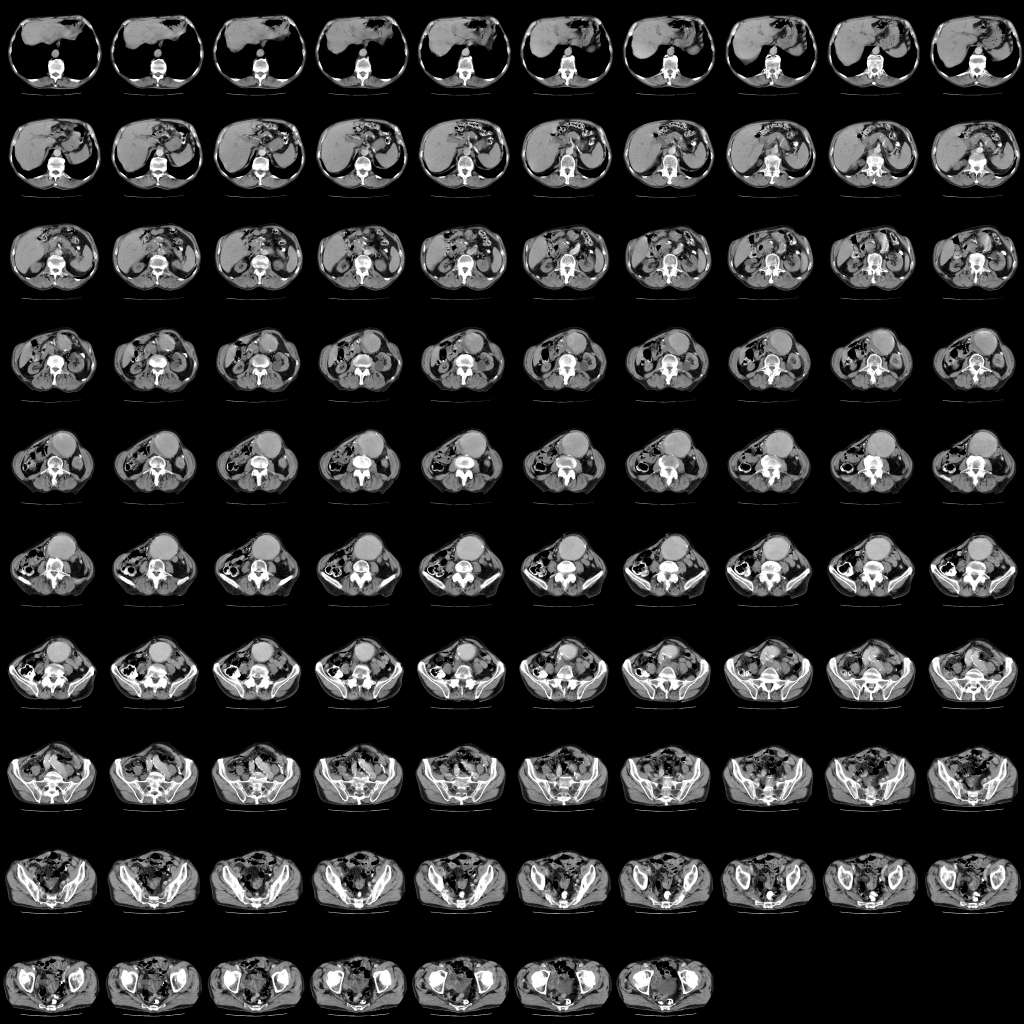
\includegraphics[width=0.4\linewidth]{./texture.jpg}
		\caption{An illustration of the 2D texture}
		\label{fig:texture}
	\end{center}
\end{figure}
The main idea is to place the binary reconstruction data in layers into the texture what then looks like shown in figure \ref{fig:texture} \footnote{Source: http://demos.vicomtech.org/volren/}. This means that we have to set a texel to black when we carve a way its corresponding voxel in the reconstruction. Another problem with the texture is that typically the number of texels doesn't sum up to a power of 2. This is solved by scaling the image with the correct amount of texels to a size of $1024 \times 1024$ which we found is the largest texture reliably generated on an android phone.

In the fragment shader we have to calculate the lookup position within the texture from 3D coordinates. We start this by calculating in which layer we are and locating this layer within the texture. Then we just have to get the correct location within the given layer.

%------------------------------------------------------------------------
\section{Conclusions}

%-------------------------------------------------------------------------
\subsection{Advantages of a mobile solution}

We blable about how nice it is that it is all on the phone now... yay!

%-------------------------------------------------------------------------
\subsection{Possible Improvements}

We tell them what part we screwed up (Multithreading, etc.) As in the presentation.

%-------------------------------------------------------------------------
\subsection{Limitations}

We talk about the problem that only the visual hull can be reconstructed using this technique and that voxel carving would be so much nicer but probably not feasible.


{\small
\bibliographystyle{ieee}
\bibliography{egbib}
}

\end{document}
